\documentclass{standalone}
\usepackage{tikz}
\usepackage{pgfplots}
\pgfplotsset{compat=1.11}
\begin{document}
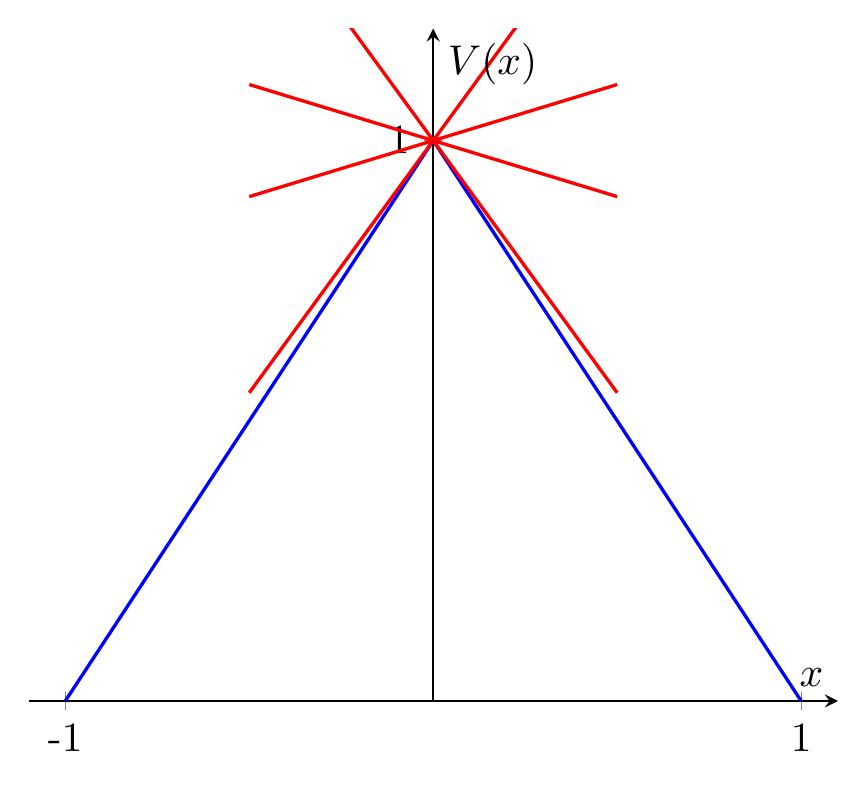
\begin{tikzpicture}[scale=1.5]
\begin{axis}[
xmin=-1.1,
xmax=1.1,
ymin=-0.,
ymax=1.2,
grid=none,
axis lines=middle,
xlabel={$x$},          
ylabel={$V(x)$},   
yticklabels={0,1},
ytick={0,1},            
xticklabels={-1,0,1},
xtick={-1,0,1}, 
]
\addplot[blue,thick,domain=-1:1]({x},{1-abs(x)});
\addplot[red,thick,domain=-0.5:.5]({x},{1+0.2*x});
\addplot[red,thick,domain=-0.5:.5]({x},{1-0.2*x});
\addplot[red,thick,domain=-0.5:.5]({x},{1-0.9*x});
\addplot[red,thick,domain=-0.5:.5]({x},{1+0.9*x});

\end{axis}
\end{tikzpicture}

\end{document}